\chapter{Logarithm}
\textbf{Definition:} A number $x$ is called the logarithm of a number $y$ to the base $b$ if $b^x = y$, where $b > 0, b\neq 1, y > 0$.

\noindent Mathematically, it is represented by the equation $\log_b y = x$ or $b^x = y$.

\textbf{Notes:}
\begin{enumerate}
\item The conditions $b>0, b\neq 1$ and $y>0$ are necessary in the definition of logarithm.
\item When $b=1$ suppose logarithm is defined, and we have to find the value of $\log_1y$. Let
  $\log_1y=x\Rightarrow 1^x=y\Rightarrow 1=y$.

  If $\log_12$ is defined then $1 = 2$. So we see that $b = 1$ leads to meaningless results. Similarly, it is true for $b \neq 1$.
\item Similarly if $y < 0$, then $b^x = y$, which is meaningless as L.H.S. is positive while R.H.S. is negative.
\item Let the condition to be true when $b = 0$. Thus, $0^x = y\Rightarrow 0 = y$. Thus, if $\log_0 2$ is defined then $0 =
  2$. Hence, our assumption leads to failure.
\item No number can have two different logarithms to a given base. Assume that a number $N$ has two different logarithms $x$ and
  $y$ with base $b$. Then, $\log_b N = x$ and $\log_b N = y$

  $\Rightarrow N = b^x$ and $N = b^y$

  $\Rightarrow b^x = b^y \Rightarrow x = y$
\item When the number or base is negative the value of logarithm comes out to be a complex number with non-zero imaginary part.

  Let $\log_e(-5) = x \Rightarrow \log_e(5.e^{i\pi}) = x$ (In complex numbers $e^{i\pi} = -1$)

  $x = \log_e5 + i\pi$
\end{enumerate}

\section{Important Results}
\begin{enumerate}
\item $\log_b 1 = 0$

  \textbf{Proof:} Let $\log_b 1 = x\Rightarrow b^x = 1 \Rightarrow x = 0$
\item $\log_b b = 1$

  \textbf{Proof:} Let $\log_b b = x \Rightarrow b^x = b \Rightarrow x = 1$
\item $b^{\log_b N} = N$

  \textbf{Proof:} Let $\log_b N = x\Rightarrow b^x = N \Rightarrow b^{\log_b N} = N$
\end{enumerate}
\section{Important Formulas}
\begin{enumerate}
\item $\log_b(x.y) = \log_bx + \log_by, (x>0, y>0)$

  \textbf{Proof:} Let $\log_bx = m \Rightarrow b^m = x$. Similarly, $b^n = y$

  $xy = b^{m + n} = b^o$ (say)

  $m + n = o \Rightarrow \log_b(x.y) = \log_bx + \log_by$

  \textbf{Corollary:} $\log_b(xyz) = \log_bx + \log_by + \log_bz$

  If $x, y < 0,$ then $\log_b(x.y) = \log_b|x| + \log_b|y|$
\item $\log_b\left(\frac{x}{y}\right) = \log_b x - \log_b y, (x, y > 0)$

  \textbf{Proof:} Let $\log_bx = m \Rightarrow b^m = x$ and $\log_by = n \Rightarrow b^n = y$

  $\frac{x}{y} = b^{m - n}$ and $\log_b\left(\frac{x}{y}\right) = o \Rightarrow b^o = \frac{x}{y}$

  $\Rightarrow m - n = o \Rightarrow \log_b\left(\frac{x}{y}\right) = \log_b x - \log_b y$

  $\log_b\left(\frac{x}{y}\right) = \log_b|x| - \log_b|y|, (x, y < 0)$
\item $\log_bN^k = k\log_b N$

  \textbf{Proof:} Let $\log_bN = x \Rightarrow b^x = N$

  Let $\log_bN^k = y \Rightarrow b^y = N^k \Rightarrow b^y = b^{kx} \Rightarrow y = kx$

  $\Rightarrow \log_bN^k = k\log_b N$
\item $\log_ba = \log_ca\log_bc$

  \textbf{Proof:} Let $\log_ba = x \Rightarrow b^x = a$

  $\log_ca = y \Rightarrow c^y = a$

  $\log_bc = z \Rightarrow b^z = c$

  $b^x = a = c^y = b^{yz} \Rightarrow x = yz \Rightarrow \log_ba = \log_ca\log_bc$

  Alternatively, we can also write it as $\log_ba = \frac{\log_ca}{\log_cb}$
\item $\log_{b^k}N = \frac{1}{k}\log_bN[b > 0]$

  \textbf{Proof:} From previous item we can infer that $\log_{b^k}N = \frac{\log N}{\log b^k} = \frac{1}{k}\log_bN$

  $\log_{b^k}N = \frac{1}{k}\log_{|b|}N[b< 0, k = 2m, m\in N]$
\item $\log_ba = \frac{1}{\log_ab}$

  \textbf{Proof:} Let $\log_ba = x \Rightarrow b^x = a$

  Also let $\log_ab = y \Rightarrow a^y = b = a^{xy} \Rightarrow xy = 1$

  $\Rightarrow \log_ba = \frac{1}{\log_ab}$
\end{enumerate}

\section{Bases of Logarthims}
There are two popular bases for logarithms. Common base is $10$ and another is $e$. When base is $10$, logarithm is known as
\textit{common logarithm} and when base is $e$, logarithm is known as \textit{natural} or \textit{Napierian logarithm}.

$\log_{10}x$ is also written as $lg~x$ and $\log_ex$ as $ln~x$.

\section{Characteristics and Mantissa}
Typically a logarithm will have an integral part and a fractional part. The integral part is called \textit{characteristics} and
fractional part is called \textit{mantissa}.

For example, if $\log x = 4.7$ then $4$ is characteristics and $.7$ is mantissa of logarithm. If characteristics is less that zero
then at times it is written with a bar above it. For example, $\log x=-5.3=\overline{5}.3$

As you can easily figure out the number of possitive integers having base $b$ and characteristics $n$ is $b^{n + 1} - b^n$.

\section{Inequality of Logarithms}
If $b > 1$ and $\log_bx_1 > \log_bx_2$ then $x_1 > x_2$. If $b < 1$ and $\log_bx_1 > \log_bx_2$ then $x_1 < x_2$.

\section{Expansion of Logarithm and Its Graph}
The logarithm series is given below:

$$\log(1 + x) = x - \frac{x^2}{2} + \frac{x^3}{3} - \frac{x^4}{4} + \ldots$$

\begin{figure}[H]
\begin{center}
  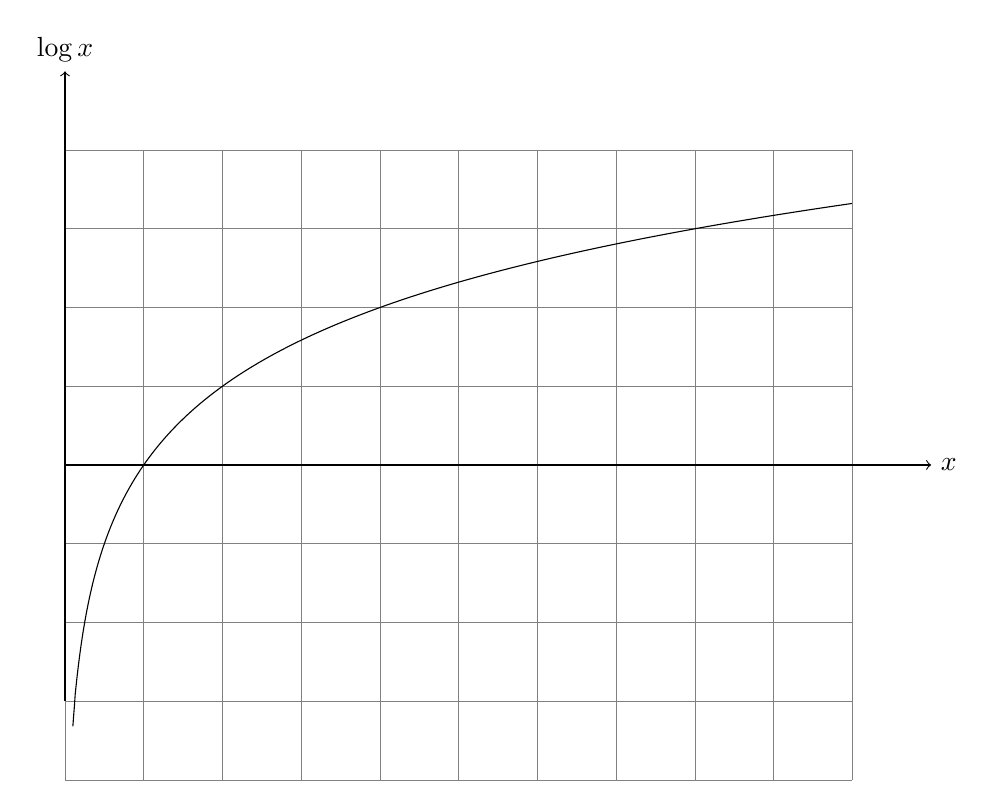
\begin{tikzpicture}
    \draw [help lines] (0,-4) grid [step=1] (10,4);
    \draw (0,0) -- (10,0);
    \draw[->] (0, 0) -- (11, 0) node[right] {$x$};
    \draw[->] (0, -3) -- (0, 5) node[above] {$\log x$};
    \draw plot [domain=0.1:10,samples=1000] (\x,{log2(\x)});
  \end{tikzpicture}
  \caption{Graph of $\log 2$}
\end{center}
\end{figure}

So we can see that rate of increment of logarithm function decreases. Rate of increment of logarithm function is given by
$\frac{1}{x}$ at any point $x$, as we will learn when we study Calculus and derivatives.

\section{Problems}
\begin{enumerate}
\item Find the value of $x$, where $\log_{\sqrt{8}} x = \frac{10}{3}$.
\item Prove that $\log_ba.\log_cb.\log_ac = 1$.
\item Prove that $\log_3\log_2\log_{\sqrt{5}}625 = 1$.
\item If $a^2 + b^2 = 23ab$, then prove that $\log\tfrac{a + b}{5} = \frac{1}{2}(\log a + \log b)$.
\item Prove that $7\log\frac{16}{15} + 5\log\frac{25}{24} + 3\log\frac{81}{80} = \log 2$.
\item Find the value of $\log\tan1^\circ + \log\tan2^\circ + \ldots + \log\tan89^\circ$.
\item Evaluate $\log_9\tan\frac{\pi}{6}$.
\item Evaluate $\frac{\log_{a^2}b}{\log_{\sqrt{a}}b^2}$.
\item Evaluate $\log_{\sqrt{5}}.008$.
\item Evaluate $\log_{2\sqrt{3}}144$.
\item Prove that $\log_3\log_2\log_{\sqrt{3}}81 = 1$.
\item Prove that $\log_ax\log_by = \log_bx\log_ay$.
\item Prove that $\log_2\log_2\log_216 = 1$.
\item Prove that $\log_ax = \log_bx\log_cb\ldots\log_nm\log_an$.
\item Prove that $a^x = 10^x\log_{10}a$.
\item If $a^2 + b^2 = 7ab$, prove that $\log\left\{\tfrac{1}{3}(a + b)\right\} = \frac{1}{2}(\log a + \log b)$.
\item Prove that $\frac{\log a\log_ab}{\log b\log_ab} = -\log_ab$.
\item Prove that $\log(1 + 2 + 3) = \log 1 + \log 2 + \log 3$.
\item Prove that $2\log(1 + 2 + 4 + 7 + 14) = \log 1 + \log 2 + \log 4 + \log 7 + \log 14$.
\item Prove that $\log 2 + 16\log\frac{16}{15} + 12\log\frac{25}{24} + 7\log\frac{81}{80} = 1$.
\item Simplify $\frac{\log_911}{\log_513}\div\frac{\log_311}{\log_{\sqrt{5}}}13$.
\item Simplify $3^{\sqrt{\log_32}} - 2^{\sqrt{\log_23}}$.
\item Find the least integer $n$ such that $7^n > 10^5$, given that $\log_{10}343 = 2.5353$.
\item If $a, b, c$ are in G.P., prove that $\log_ax, \log_bx, \log_cx$ are in H.P.
\item Prove that $\log\sin8x = 3\log2 + \log\sin x + \log\cos x + \log\cos2x + \log\cos4x$.
\item If $x = \log_{2a}a, y = \log_{3a}2a$ and $z = \log_{4a}3a$ then prove that $xyz + 1 = 2yz$.
\item If $a$ and $b$ are the lengths of the sides and $c$ be the length of the hypotenuse of a right-angle triangle and $c - b \neq
  1$ and $c + b\neq 1$, prove that $\log_{c + b}a + \log_{c - b}a = 2\log_{c + b}a\log_{c - b}a$.
\item If $\frac{\log x}{y - z} = \frac{\log y}{z - x} = \frac{\log z}{x - y}$, then prove that $x^xy^yz^z = 1$.
\item If $\frac{yz\log(yz)}{y + z} = \frac{zx\log(zx)}{z + x} = \frac{xy\log(xy)}{x + y}$, prove that $x^2 = y^y = z^2$.
\item Prove that $(yz)^{\log y - \log z}(zx)^{\log z - \log x}(xy)^{\log x - \log y} = 1$.
\item Prove that $\frac{1}{\log_2N} + \frac{1}{\log_3N} + \ldots + \frac{1}{\log_{1988}N} = \frac{1}{\log_{1988!}N}$.
\item If $0<x<1$, prove that $\log(1 + x) + \log(1 + x^2) + \log(1 + x^4) + \ldots$ to $\infty = -\log(1 - x)$.
\item Find the sum of the series $\frac{1}{\log_2a} + \frac{1}{\log_4a} + \ldots$ up to $n$ terms.
\item If $\log_410 = x, \log_220 = y$ and $\log_58 = z$, prove that $\frac{1}{x + 1} + \frac{1}{y + 1} + \frac{1}{z + 1} = 1$.
\item If $x = \log_abc, y = \log_bca, z = \log_cab$, prove that $\frac{1}{x + 1} + \frac{1}{y + 1} + \frac{1}{z + 1} = 1$.
\item Prove that $\frac{1}{1 + \log_ba + \log_bc} + \frac{1}{1 + \log_ca + \log_cb} + \frac{1}{1 + \log_ab + \log_ac} = 1$.
\item Prove that $x^{\log y - \log z}y^{\log z - \log x}z^{\log x - \log y} = 1$.
\item If $\frac{\log a}{y - z} = \frac{\log b}{z - x} = \frac{\log c}{x - y}$, prove that $a^xb^yc^z = 1$.
\item If $\frac{x(y + z - x)}{\log x} = \frac{y(z + x - y)}{\log y} = \frac{z(x + y - z)}{x - y}$, prove that $y^zz^y = z^xx^z =
  x^yy^x$.
\item If $\frac{\log a}{b - c} = \frac{\log b}{c - a} = \frac{\log c}{a - b},$ prove that $a^{b + c}b^{c + a}c^{a + b} = 1$.
\item If $\frac{\log x}{q - r} = \frac{\log y}{r - p} = \frac{\log z}{p - q}$, prove that $x^{q + r}y^{r + p}z^{p + q} =
  x^py^qz^r$.
\item If $y = a^{\frac{1}{1 - \log _ax}}$ and $z = a^{\frac{1}{1 - \log_ay}}$, prove that $x = a^{\frac{1}{1 - \log_az}}$.
\item Let $f(x) = \frac{1}{1 - \log_ex}$, $f(y) = e^{f(z)}$ and $z = e^{f(x)}$, prove that $x = e^{f(y)}$.
\item Show that $\frac{1}{\log_2n} + \frac{1}{\log_3n} + \frac{1}{\log_4n} + \ldots + \frac{1}{\log_{43}n} =
  \frac{1}{\log_{43!}n}$.
\item Show that $2(\log a + \log a^2 + \log a^3 + \ldots + \log a^n) = n(n + 1)\log a$.
\item Find the number of digits in $12^{12}$, without actual computation. [Given $\log 2 = 0.301$ and $\log 3 = 0.477$]
\item How many positive integers have a characteristics of $2$ when base is $3$.
\item Prove that $\log_ax\log_by = \log_bx\log_ay$.
\item If $a, b, c$ are in G.P., prove that $\log_ax, \log_bx, \log_cx$ are in H.P.
\item How many zeros are there between the decimal point and first significant digit in $0.0504^{10}?$ Given $\log 2 = 0.301, \log
  3 = 0.477, \log 7 = 0.845$.
\item Find the number of digits in $72^{15}$ without actual computation. Given $\log 2 = 0.301$ and $\log  3 = 0.477$.
\item How many positive integers have characteristics $2$ when base is $5$?
\item If $\log 2 = 0.301$ and $\log 3 =0.477$, find the number of digits in $3^{15}\times 2^{10}$.
\item If $\log 2 = 0.301$ and $\log 3 =0.477$, find the number of digits in $6^{20}$.
\item If $\log 2 = 0.301$ and $\log 3 =0.477$, find the number of digits in $5^{25}$.
\item Solve $\log_a[1 + \log_b\{1 + \log_c(1 + \log_px)\}] = 0$.
\item Solve $\log_7\log_5(\sqrt{x + 5} + \sqrt{x}) = 0$.
\end{enumerate}

\noindent Solve the following equations:

\begin{enumerate}[resume]
\item $\log_2x + \log_4(x + 2) = 2$.
\item $\log_{x + 2}x + \log_x(x + 2) = \frac{5}{2}$.
\item $\log(x + 1) = 2\log x$.
\item $2\log_xa + \log_{ax}a + 3\log_{a^2x}a = 0.$ Given $a > 0$.
\item $x + \log_{10}(1 + 2^x) = x\log_{10}5 + \log_{10}6$.
\item $x^{\tfrac{3}{4}(\log_2x)^2 + \log_x{2 - \tfrac{5}{4}}} = \sqrt{2}$.
\item $(x^2 + 6)^{\log_3x} = (5x)^{\log_3x}$.
\item $(3 + 2\sqrt{2})^{x^2 - 6x + 9} + (3 - 2\sqrt{2})^{x^2 - 6x + 9} = 6$.
\item $\log_8\left(\tfrac{8}{x^2}\right)\div(\log_8x)^2 = 3$.
\item $\sqrt{\log_2(x)^4} + 4\log_4\sqrt{\tfrac{2}{x}} = 2$.
\item $2\log_{10}x - \log_x0.01 = 5$.
\item $\log_{\sin x}2\log_{\cos x}2 + \log_{\sin x}2 + \log_{\cos x}2 = 0$.
\item $2^{x + 3} + 2^{x+2} + 2^{x + 1} = 7^x + 7^{x - 1}$.
\item $\log_{\sqrt{2}\sin x}(1 + \cos x) = 2$.
\item $\log_{10}[198 + \sqrt{x^3 - x^2 - 12x + 36}] = 2$.
\item If $\log 2 = 0.30103$ and $\log 3 = 0.47712,$ solve the equation $2^x3^{2x} - 100 = 0$.
\item $\log_x3\log_{\frac{x}{3}}3 + \log_{\frac{x}{81}}3 = 0$.
\item $\log_{(2x + 3)}(6x^2 + 23x + 21) = 4 - \log_{(3x + 7)}(4x^2 + 12x + 9)$.
\item $\log_2(x^2 - 1) = \log_{\frac{1}{2}}(x - 1)$.
\item $\log_5\left(5^{\tfrac{1}{x} + 125}\right) = \log_56 + 1 + \frac{1}{2x}$.
\item $\log_{100}|x + y| = \frac{1}{2}$ and $\log_{10}y - \log_{10}|x| = \log_{100}4$.
\item $2\log_2\log_2x + \log_{\tfrac{1}{2}}\log_2(2\sqrt{2}x) = 1$.
\item $\log_{\tfrac{3}{4}}\log_8(x^2 + 7) + \log_{\tfrac{1}{2}}\log_{\tfrac{1}{4}}(x^2 + 7)^{-1} = 2$.
\item $\log_{10}x + \log_{10}x^{\tfrac{1}{2}} + \log_{10}x^{\tfrac{1}{4}} + \ldots$ to $\infty = y$ and $\frac{1 + 3 + 5 + \ldots +
  (2y - 1)}{4 + 7 + 10 + \ldots + (3y + 1)} = \frac{20}{7\log_{10}x}$.
\item $18^{4x - 3} = (54\sqrt{2})^{3x - 4}$.
\item $4^{\log_93} + 9^{\log_24} = 10^{\log_x83}$.
\item $3^{4\log_9(x + 1)} = 2^{2\log_2(x + 3)}$.
\item $\frac{6}{5}a^{\log_ax\log_{10}a\log_a5} - 3^{\log_{10}\tfrac{x}{10}} = 9^{\log_{100}x + \log_42}$.
\item $2^{3x + \frac{1}{2}} + 2^{x + \frac{1}{2}} = 2^{\log_26}$.
\item $(5 + 2\sqrt{6})^{x^2 - 3} + (5 - 2\sqrt{6})^{x^2 - 3} = 10$.
\item For $x> 1$, show that $2\log_{10x}x - \log_x{.01}\geq 4$.
\item Show that $|\log_b a + \log_ab| > 2$.
\item Solve $\log_{0.3}(x^2 + 8) > log_{0.3}9x$.
\item Solve $\log_{x - 2}(2x - 3) > \log_{x - 2}(24 - 6x)$.
\item Find the interval in which $x$ will lie if $\log_{0.3}(x - 1) < \log_{0.09}(x - 1)$.
\item Solve $\log_{\tfrac{1}{2}}x \geq \log_{\tfrac{1}{3}}x$.
\item Solve $\log_{\tfrac{1}{3}}\log_4(x^2 - 5) > 0$.
\item Solve $\log(x^2 -2x -2)\leq 0$.
\item Solve $\log_2^2(x-1)^2 - \log_{0.5}(x - 1) > 5$.
\item Prove that $\log_217\log_{\tfrac{1}{5}}2\log_3\tfrac{1}{5} > 2$.
\item Show that $\log_{20}3$ lies between $\frac{1}{2}$ and $\frac{1}{3}$.
\item Show that $\log_{10}2$ lies between $\frac{1}{4}$ and $\frac{1}{3}$.
\item Solve $\log_{0.1}(4x^2 - 1) > \log_{0.1}3x$.
\item Solve $\log_2(x^2 - 24) > \log_25x$.
\item Show that $\frac{1}{\log_3\pi} + \frac{1}{\log_4\pi} > 2$.
\item Without actual computation find greater among $(0.01)^{\tfrac{1}{3}}$ and $(0.001)^{\tfrac{1}{5}}$.
\item Without actual computation find greater among $\log_23$ and $\log_311$.
\item Solve $\log_3(x^2 + 10) > \log_37x$.
\item Solve $x^{\log_{10}x} > 10$.
\item Solve $\log_2x\log_{2x}2log_24x > 1$.
\item Solve $\log_2x\log_32x + \log_3x\log_24x > 0$.
\item Find the value of $\log_{12}60$ if $\log_630 = a$ and $\log_{15}24 = b$.
\item If $\log_ax, \log_bx$ and $\log_cx$ are in A.P. and $x\neq 1$, prove that $c^2 = (ac)^{\log_ab}$.
\item If $a = \log_{\tfrac{1}{2}}\sqrt{0.125}$ and $b = \log_3\left(\frac{1}{\sqrt{24} - \sqrt{17}}\right)$ then find whether $a >0,
  b> 0$.
\item Which one is greater among $\cos(\log_e\theta)$ and $\log_e(\cos\theta)$ if $e^{-\tfrac{\pi}{2}} < \theta < \frac{\pi}{2}$.
\item If $\log_2x + \log_2y \geq 6$, prove that $x + y\geq 16$.
\item If $a,b,c$ eb three distinct positive numbers, each different from $1$ such that $\log_ba\log_ca - \log_qaa + \log_ab\log_cb
  - \log_bb + \log_ac\log_bc - \log_cc = 0$.
\item If $y = 10^{\tfrac{1}{1 - \log x}}$ and $z = 10^{\tfrac{1}{1 - \log y}}$, prove that $x = 10^{\tfrac{1}{1 - \log z}}$.
\item If $n$ is a natural number such that $n = p_1^{a_1}p_2^{a_2}p_3^{a_3}\ldots p_k^{a_k}$ and $p_1, p_2, p_3, \ldots, p_k$ are
  distinct primes, then show that $\log n\geq k\log 2$.
\item The numbers $3, 3\log_yx, 3\log_zy, 7\log_xz$ form and A.P. then prove that $x^{18} = y^{21} = z^{28}$.
\item Prove that $\log_418$ is an irrational number.
\item If $x, y, z> 1$ are in G.P. then prove that $\frac{1}{1+ \ln x}, \frac{1}{1 + \ln y}, \frac{1}{1 + \ln z}$ are in H.P.
\item Find the value of $\log_{30}8$, if $\log_{30}3 = a$ and $\log_{30}5 = b$.
\item Find the value of $\log_{54}168$, if $\log_712 = a$ and $\log_{12}24 = b$.
\item If $a\neq 0$ and $\log_x(a^2 + 1) < 0$ then find the interval in which $x$ lies.
\item If $\log_{12}18 - a$ and $\log_{24}54=b$, prove that $ab + 5(a - b) = 1$.
\item If $a,b,c$ are in G.P., show that $\log_ax, \log_bx, \log_cx$ are in H.P.
\item If $a, a_1, a_2, \ldots, a_n$ are in G.P. and $b, b_1, b_2, \ldots, b_n$ in A.P. with positive terms and also the common
  difference of A.P. and common rations of G.P. are positive, show that there exists a system of logarithm for which $\log a_n -
  b_n = \log a - b$ for any $n$. Find the base of this system.
\item If $\log_32, \log_3(2^x - 5)$ and $\log_3\left(2^x - \frac{7}{2}\right)$ are in A.P., find the value of $x$.
\item Prove that $\log_27$ is an irraational number.
\item If $\log_{0.5}(x - 2) < \log_{0.25}(x - 2)$, then find the interval in which $x$ lies.
\end{enumerate}
